% !TeX spellcheck = en_GB

\section{Association Analysis}

\begin{breakbox}
\boxtitle{Candidate Generation:}
\begin{itemize}
	\item Set minimum support.
	\item Identify frequent 1-itemsets.
	\item Combine to frequent multi-itemsets.
	\item Build possible 2-itemsets.
	\item Determine frequency of 2-itemsets.
	\item non-frequent itemsets are eliminated.
	\item Build possible 3-itemsets.
	\item Candidate elimination.
	\item Determine frequency of remaining candidates.
	\item Build possible 4-itemsets, and so on \ldots
\end{itemize}
\end{breakbox}

\begin{breakbox}
\boxtitle{A-Priori Algorithm:}
\begin{itemize}
	\item Candidate generation (see above).
	\item set minimum confidence $\gamma$.
	\item for each frequent itemset: set up every possible combination as a rule.
	\item calculate confidence for every rule.
	\item select rules $\geq$ minimum confidence.
\end{itemize}
\end{breakbox}

\begin{breakbox}
\boxtitle{FP Growth:}
\newline Algorithm:
\begin{itemize}
	\item Step 1: full table scan and determination of support count for 1-item-sets.
	\item Step 2:
		\begin{itemize}
			\item select items with at least minimum support.
			\item sort items by support count in descending order / corresponds to a reordering of columns (projection).
			\item table is processed in that order.
		\end{itemize}
	\item Step 3: Generating an FP-tree:
		\begin{itemize}
			\item create empty root node.
			\item for each transaction in reordered table:
				\begin{itemize}
					\item add a new branch to the tree.
					\item nodes of this branch correspond to the sequence of attributes in the reordered table.
					\item existing parts of branches (prefixes) will not be created but a counter on each node in the prefix is incremented by 1.
				\end{itemize}
			\item for quick tree traversals
				\begin{itemize}
					\item additional item header table: For each item it holds pointers to every node containing that item.
				\end{itemize}
		\end{itemize}
	\item Step 4: Mining the FP-tree:
		\begin{itemize}
			\item Start with the least frequent item (last column in the reordered table).
			\item For each frequent item.
				\begin{itemize}
					\item generate its conditional pattern base, i.e. a list of all existing paths in the tree leading to that item (all prefixes).
					\item generate its conditional FP-tree, i.e. all frequent enough ($\geq$ minimum support) paths leading to the item in the conditional pattern base (frequent prefixes).
					\item combine each frequent prefix with the item itself (the suffix), forming a frequent pattern.
				\end{itemize}
			\item continue with next item in reversed table order.
		\end{itemize}
\end{itemize}
Exercise: Identify frequent itemsets with minimum support = 0.2, employing the FP-growth method.
\begin{center}
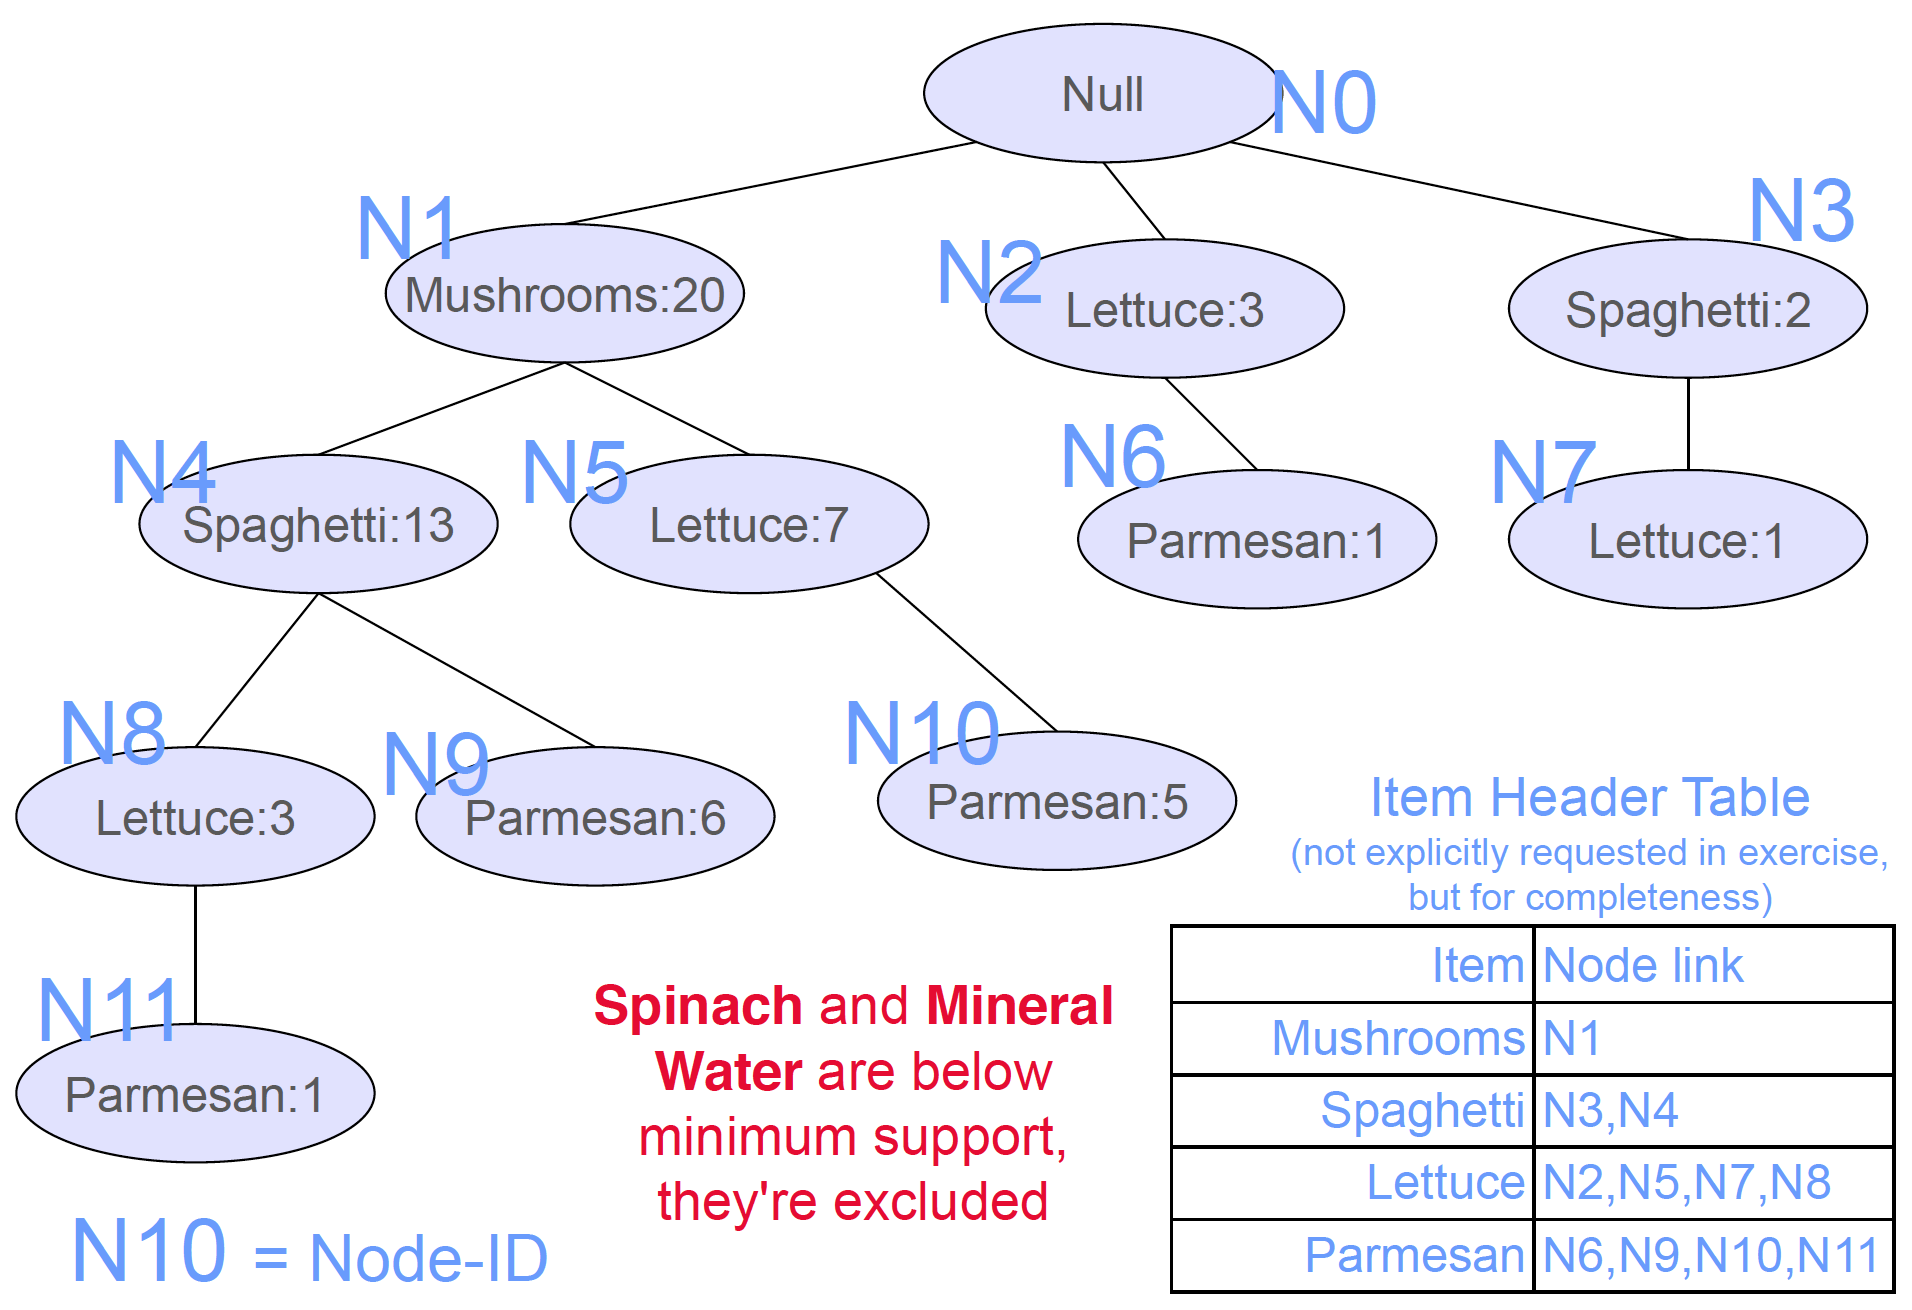
\includegraphics[width=.15\textwidth]{slides_images/fp_tree}
\end{center}
This results in the following table:
\begin{center}
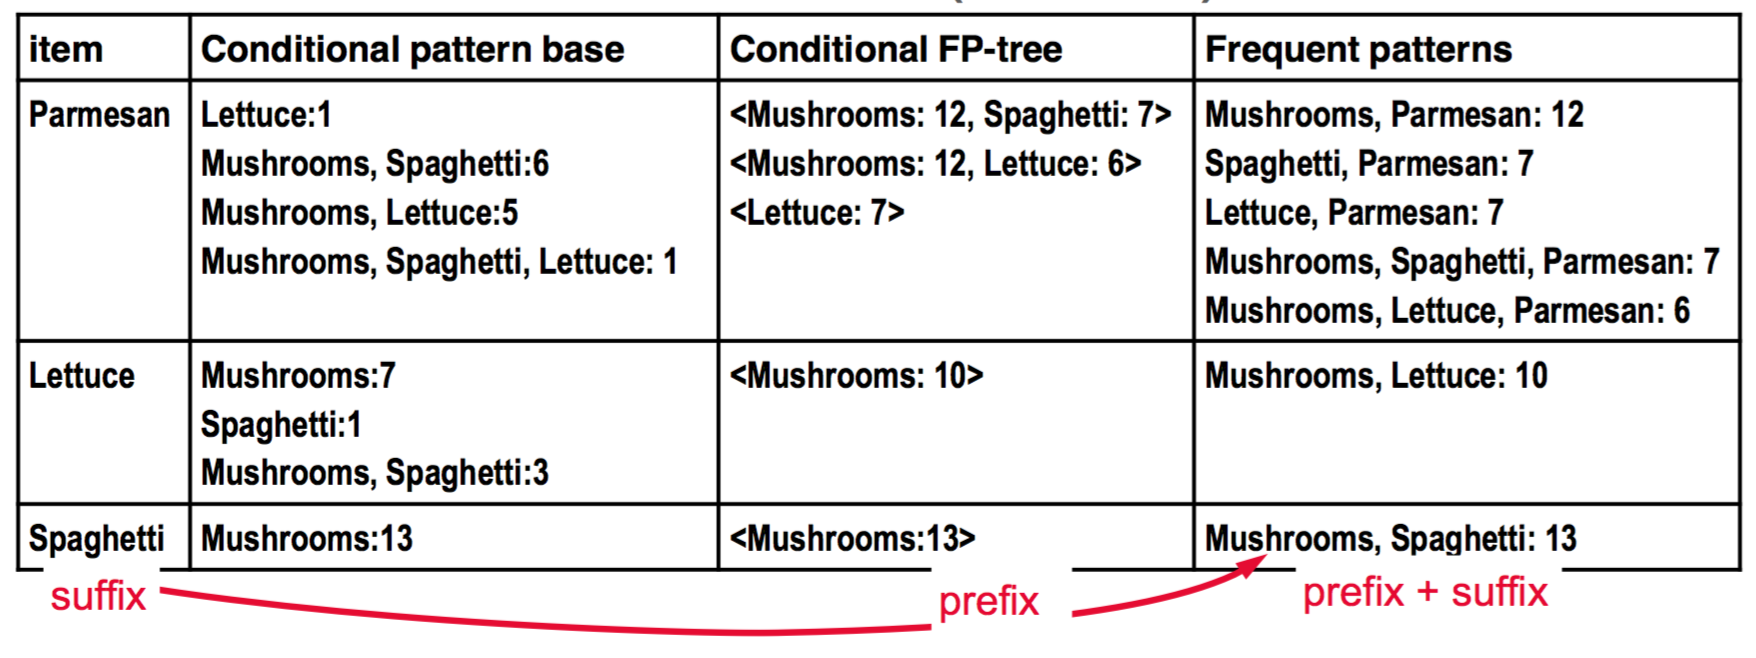
\includegraphics[width=.15\textwidth]{slides_images/frequent_patterns}
\end{center}
\end{breakbox}

\begin{breakbox}
\boxtitle{Support \& Confidence:}
\begin{itemize}
	\item Rule: R: A $\Rightarrow$ B
	\item Support (Reflects the significance, the importance of an itemset):
		\begin{itemize}
			\item[] supp(A) $= \frac{\text{\#transactions with A}}{\text{total \#transactions}}$
			\item[] supp(R) $= \frac{\text{\#transactions with A} \cup \text{B}}{\text{total \#transactions}}$
		\end{itemize}
	\item Confidence (Reliability measure, how certain am I to say, that B will occur given that A is present.):
		\begin{itemize}
			\item[] conf(R) $= \frac{\text{supp(R)}}{\text{supp(A)}}$
			\item[] conf(R) $= \frac{\text{\#transactions with A} \cup \text{B}}{\text{\#transactions with A}}$
		\end{itemize}
\end{itemize}
\end{breakbox}

\begin{breakbox}
\boxtitle{Correlation \& Lift:}
\begin{itemize}
	\item Correlation (Reflects the significance, the importance of an itemset):
		\begin{itemize}
			\item[] corr$_\text{A,B} = \frac{\text{P(A} \cup \text{B)}}{\text{P(A)} \cdot \text{P(B)}}$
			\item correlation $>$ 1: positively correlated, A implies presence of B.
			\item correlation $<$ 1: negatively correlated, A implies absence of B.
		\end{itemize}
	\item Lift (correlation measure in market basket analysis often referred to as lift) How much times is $A\leftarrow B$ better than the known average:
		\begin{itemize}
			\item[] lift(A $\rightarrow$ B) $= \frac{\text{conf(A} \rightarrow \text{B)}}{\text{supp(B)}}$
			\item Note: lift(A $\rightarrow$ B) = corr$_\text{A,B}$ (insert definition of conf in lift).
			\item lift tells us how much the rule's confidence exceeds mere probability.
			\item lift indicates a rule's overall significance.
		\end{itemize}
\end{itemize}
\end{breakbox}

\begin{breakbox}
\boxtitle{Limits To Association Analysis:}
\begin{itemize}
	\item Rules inherent to the data are of no use.
	\item Not all rules are interesting.
	\item Rules might induce wrong associations.
	\item Rules might be nonsense.
\end{itemize}
\end{breakbox}
